% !TeX root = RJwrapper.tex
\title{Ordinal Regression Diagnostics in R: An Introduction to the ordr package}
\author{by Brandon M. Greenwell, Author Two and Author Three}

\maketitle

\abstract{
An abstract of less than 150 words.
}

\section{Introduction}

Coming soon!

Ordinal regression (OR) models...


\subsection{Ordinal regression}

Coming soon!

\begin{itemize}
  \item Provide brief background on OR models.
  \item Provide brief background on relevant packages.
\end{itemize}


\subsection{Li-Shepherd residuals}

Coming soon! These are available in package \CRANpkg{rms}.


\subsection{Surrogate-based residuals}

Coming soon!


\subsubsection{Graphical properties}

Coming soon!


\section{Residual-based OR diagnostics in R}

Coming soon!

\begin{example}
  library(MASS)
  houses.polr <- polr(Sat ~ Infl + Type + Cont, weights = Freq, data = housing)
\end{example}

Talk about model.

\begin{example}
  res <- resids(houses.polr)
\end{example}


\subsection{Drawing multiple samples}

\begin{example}
  res <- resids(houses.polr, nsim = 50)
\end{example}


\subsection{Detecting heteroscedasticty}

For this example, we generated $n = 2000$ observations from the following ordered probit model:
\begin{equation*}
  Pr\left\{\mathcal{Y} \le j\right\} = \Phi\left\{\left(\alpha_j + \beta X\right) / \sigma_X\right\}, \quad j = 1, 2, 3, 4, 5,
\end{equation*}
where $\alpha_1 = -36$, $\alpha_2 = -6$, $\alpha_3 = 34$, $\alpha_4 = 64$, $\beta = -4$, $X \sim \mathcal{U}\left(2, 7\right)$, and $\sigma_X = X ^ 2$.

The following block of code uses the \pkg{MASS} package function \code{polr} to fit a probit model to the \code{hd} data.
\begin{example}
  library(ggplot2)
  library(MASS)
  library(ordr)
  fit.polr <- polr(y ~ x, data = hd, method = "probit")
  set.seed(101)  # for reproducibility
  sur.res <- resids(fit.polr)  # surrogate-based residuals

  # Figure 1 (left)
  ggplot(data.frame(x = hd$x, y = sur.res), aes(x, y)) +
    geom_point(size = 2, alpha = 0.25) +
    geom_smooth(color = "red", se = FALSE) +
    ylab("Surrogate residual")
\end{example}
Alternatively, we can plot the residuals directly from the fitted model using the \code{autoplot} function:
\begin{example}
  autoplot(fit.polr, what = "covariate", x = hd$x)  # plot not shown
\end{example}

We can also easily obtain and plot the standard Li-Shepherd residuals against $x$ using the \pkg{PResiduals} package function \code{presid}:
\begin{example}
  library(PResiduals)
  ls.res <- presid(fit.polr)  # probability scale residuals

  # Figure 1 (right)
  ggplot(data.frame(x = hd$x, y = ls.res), aes(x, y)) +
    geom_point(size = 2, alpha = 0.25) +
    geom_smooth(color = "red", se = FALSE) +
    ylab("Probability scale residual")
\end{example}

\begin{figure}
  \centering
  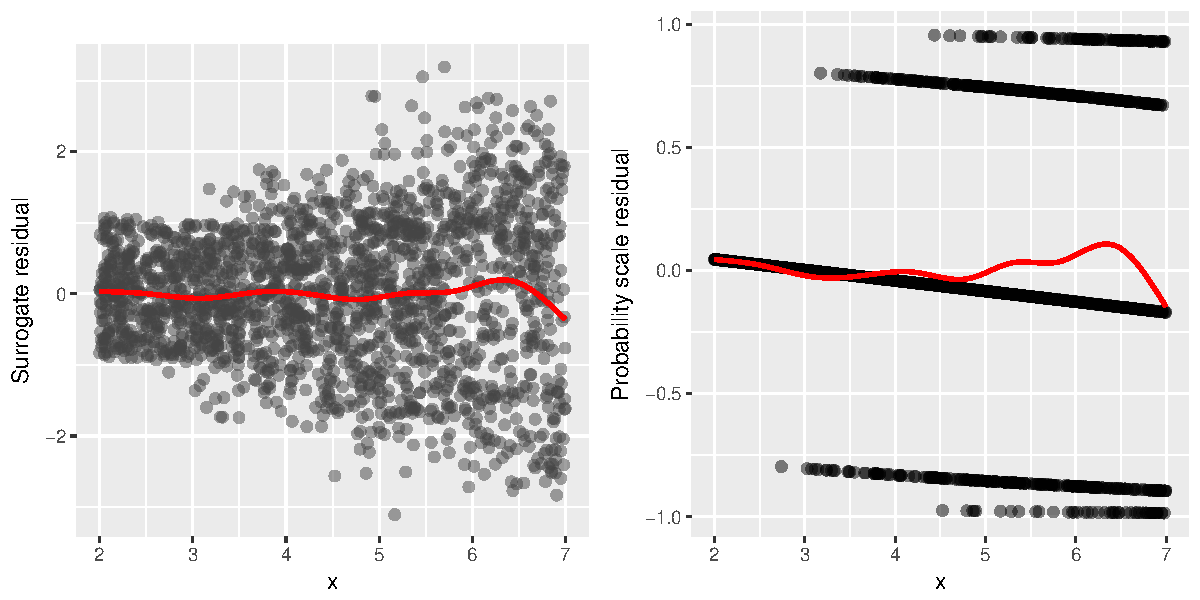
\includegraphics[width=1\textwidth]{heteroscedasticity}
  \caption{Residual vs. covariate plots for the simulated heteroscedastid data. \textit{Left}: Surrogate residuals. \textit{Right}: Probability scale residuals.}
  \label{fig:heteroscedasticity}
\end{figure}

\subsection{Detecting a misspecified mean structure}

Coming soon!


\subsection{Detecting a misspecified link function}

Coming soon!


\subsection{Checking the proportionality assumption}

Coming soon!


\subsection{Assessing goodness-of-fit}

Coming soon!

\begin{example}
  plot(gof(houses.polr, nsim = 1000))
\end{example}


\section{Summary}

This file is only a basic article template. For full details of \emph{The R Journal} style and information on how to prepare your article for submission, see the \href{https://journal.r-project.org/share/author-guide.pdf}{Instructions for Authors}.


\section{Acknowledgments}

TBD.


\bibliography{greenwell-lastname2-lastname3}

\address{Author One\\
  Affiliation\\
  Address\\
  Country\\
  (ORCiD if desired)\\
  \email{author1@work}}

\address{Author Two\\
  Affiliation\\
  Address\\
  Country\\
  (ORCiD if desired)\\
  \email{author2@work}}

\address{Author Three\\
  Affiliation\\
  Address\\
  Country\\
  (ORCiD if desired)\\
  \email{author3@work}}
